% Preamble
\documentclass[11pt]{article}
\usepackage{braket}
\usepackage{graphicx}
\usepackage[margin=1in]{geometry}

\usepackage{makeidx}  % allows for indexgeneration
\usepackage{ifpdf}
\usepackage{url}


\title{Elementary Cellular Automata as Non-Cryptographic Hash Functions}
\date{May 2025}
\author{Daniel McKinley}

% Document
\begin{document}

\maketitle

\section{Introduction}

Ten of the 256 elementary cellular automata (ECA) rules are explored as a non-cryptographic hash function using a lossy compression error-minimization function that operates on input data in 4x4 binary cells \cite{Wolfram}. The hash's key properties are that the codewords are unique and evenly distributed, has a lossy inverse, hashed data can be operated on efficiently within a hashed state, and through bitmap file processing shows a clear application to edge detection at shallow depths of iteration.  The loops parallel the nested $2^n$ structure of the Fast Fourier Transform (FFT) and Fast Walsh-Hadamard Transform. General algorithm outline, specific ECA rules, and aggregate properties are discussed. It is implemented in Java and more images and gifs and code links are available at the website\cite{dmwebsite}.\\

\section{Main Algorithm}
The hash algorithm is a kind of lossy compression that operates on 4x4 wrapped cells of binary input data that minimizes errors in compression on a small scale looped over all the input data. Within each cell, row 0 is the input neighborhood and rows 1, 2, and 3 are the ECA rule's output. All 16 possible row 0 inputs are calculated for a given input and then scored so that each bitwise discrepancy between the codeword's output and the input is summed with a weight of $2^row$. The input neighborhoods that minimize and maximize the error score are noted as the codeword pair for that 4x4 input and each codeword is 4 bits. Doing this procedure for all  $2^{16}=65536$ possible 4x4 input neighborhoods produces a truth table for a particular ECA rule.\\

\begin{center}
There are $2^{16}=65536$ binary 4x4 arrays, wrapped by column\\
$2^4$ possible $row_0$ neighborhoods for a given ECA rule\\
The ECAfunction(input) is output for rows 1, 2, 3
These 16 outputs are scored for errors by\\
Summing the discrepancies between originalInput and codewordOutput\\
Weighted by either $2^{row}$ or $2^{column}$\\
\[  \sum_{r=0}^{3} \sum_{c=0}^{3} 2^r ( compressionAttempt_{r c} \oplus original_{r c}) \]\\
 The minimizing and maximizing values of all possible input are noted\\
 as the codeword pair of the original binary matrix for a given ECA rule\\
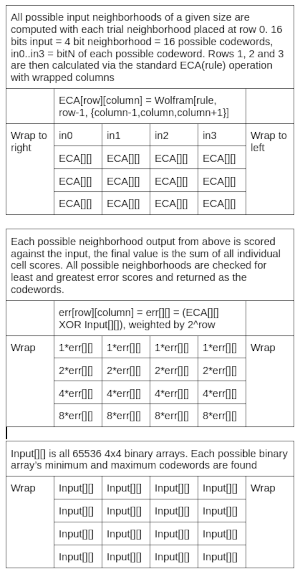
\includegraphics{fourByfour}
\end{center}

Having generated the truth table for a given ECA rule, it is applied to a 2D binary array and bitmap image as follows and with a slight variation is done for 1D input. For every (wrapped) (row,column) location in the input, the local 4x4 cell hash input is the sum of it and its neighbors $2^d$ away, $(row,column)..((row+2^d),(column+2^d))$ where d is depth of iteration. The location's value is replace with the respective minimizing or maximizing codewords that best represent its neighborhood by minimizing error. The comparing of neighbors of powers of 2 distance away is the same stucture as the FFT and Fast Walsh Transforms with rehashes instead of sums. When the iteration's neighbor distance is $log2_{row}$ or $log_2(column)$, whichever is greater, every bit has influenced every other bit and the avalanche property can be analyzed. Since every neighborhood has a unique solution, any size of any given input has a unique hash if hashing in place and not compressing.\\

\begin{center}
Below is a Fast Walsh-AlgorithmCode.Hadamard Example \cite{enwiki:1261916659}\\
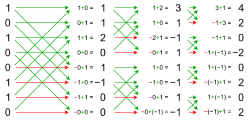
\includegraphics{FastWalshHadamard}\\
If you did the above with the powers of 2 in reverse order you would get this. \\
This the 1 dim version, and instead of a sum term it's a rehash.\\ 
Find the codewords of the codewords, twice as far apart each time.\\
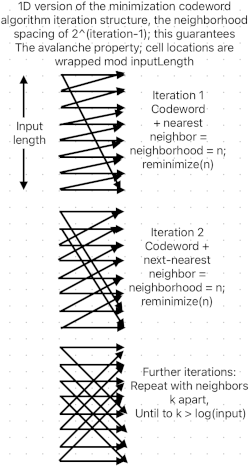
\includegraphics{AlgoStruct}\\
\end{center}

\section{Hash properties}

\subsection{Hash Function Background}

Hash functions can be described as indexing functions analogous to alphabetical order. If I give you a random word you've never heard before you can still look it up in the dictionary because they are in alphabetical order. It would be more difficult to look it up in a book ordered by numbers of letters because of conflicts when different words have the same number of letters. An extension of this idea can do the same thing for any kind of data: audio, visual, archives, and more. Media databases use hashes to index data and web servers use hashes to distribute workloads. If a site gets a billion visitors a day the work has to be divided up between sub servers by hashing certain reference data such as the client's id data. Web servers keep frequently used data closer to the top of the stack and hashes are used to save significant computing time through using bloom filters to determinine whether requested data is already up front in the cache or that a deeper database has to be called.\\

There are two kinds of hashes called cryptographic hashes and non-cryptographic hashes. Cryptographic hashes are used in password storage, encryption, and blockchain currency and other secure applications. The hashes described here are almost the opposite of cryptographic because of the transparent inverses, retroactive hashing, minimal avalanche, and linear operation component rules. Other properties that make a good hash like the avalanche property and whether it outputs a certain or fixed size output are addressed below.\\

\subsection{Two sets of Eight Rules}
Within the 256 ECA rules, there are 8 $[0,15,51,85,170,204,240,255]$ using a row weighted errorScore that have the properties of unique codewords for any given input, every codeword occurs the same number of times with relatively even distribution of codewords across the 65536 neighborhoods in the truth table.  Since every small scall solution has a unique solution every input at large scale has a single hash output. These properties apply to both errorScore minimization and errorScore maximization. \\

There is another overlapping subset of 8, $[0,15,85,90,165,170,240,255]$ whose errorScore weight is $2^{column}$ rather than $2^{row}$. Again, the codewords are distributed perfectly evenly, there are unique solutions for every input, and has a minimizing and a maximizing codeword set. These lists share a few members with the XOR-additive list. \cite{xorAdditive}. Most properties apply to both with a few exceptions.\\

0 and 255 are included because of the 4 rows of the output matrix, 1 is neighborhood input and 3 are output, and so still produce an errorScore and a unique solution. In the hashLogicOpTransform class while 255 minimizations have a valid transform in its truth table, it has to be manually overidden to zero, adding a constant to the O(N). All other rowError codewords with valid operations work seamlessly. \\

Another reason they're not completely trivial is that a complete codeword set can be encoded as trigintaduonions, hypercomplex rings with degree 5, two past octonions with 32 elements, having no negative members when using hexadecimal codewords.  There are 32 unit vectors in degree 5 quaternions, and by encoding in binary the 16th's place is the negative sign so the hexadecimal hash codewords don't produce negative trigintaduonion elements. Having a unique distinct solution, the trigintaduonions lend themselves easily to physical interpretations of the hash sets and can be an orthonormal basis for data structures and tight integration with GF($2^m$). I also propose that all degrees of quaternions, octonions, and so on in general be call nions: 4-nion, 8-nion, 16-nion and so on if the degree is called for, or possibly $nion_D$ as a subscript or nion(D), simplifying the prefixes.\\

\subsection{Input Sizes}
This algorithm can be used to make any sized hash. This hash is implemented to either hash-in-place so that the data stays the same size or as compression with the data size quartering each iteration. To implement any size output, first hash to the avalanche point as the fixed data size version, then as compression to the size desired and/or pad with zeroes at the beginning or the end. Rather than padding with zeroes one can use an inversion to expand the hash to a larger size, however inversion is more computationally expensive than compression. Another option is to hash to the avalanche point and take a subset of it. If using every minMax row-column codeword set, hash to desired size and then hash the hashes.\\

\subsection{Inverse}

There is a hexadecimal version of the hash and a single bit version of the hash. In the hexadecimal version the bitmap raster gets broken down into 4 bit chunks and the single bit version breaks down the raster into single bits. The hex version is faster and is used to generate the images and gifs; the single bit version produces better inverse loss rates. The hexadecimal versions breaking down the raster into hexadecimal display roughly the same experimental inverse as their respective codeword sets, about 3/16 . However the single-hex-single inverse codewords have a loss of about 2 percent on inversion.  \\

The inverse uses a voting system where the codeword neighborhoods add or subtract the appropriate error weight at every location in their zone of influence. The codeword is the algorithm's best guess at what the input was, so the inverse it its neighborhood's errorScore weighted best guesses at the pixels they're relevant to and are tallied and accounted for as output. A codeword votes its lossily reproduced neighborhood with the proper string of positives and negatives  for value 0..1, minimization..maximization, and rowError..columnError.\\

\subsection{Retroactive Hashing}
Hashed input can be operated on with the row weighted rule set without the original input and without inverting it. This happens through a transformation of logic operation because of the linear nature of the rules used. Rules 15, 51, and 85 simply pass the left middle or right input bit with no other operation or dependency, 170, 204, and 240 are the complements, and 90 and 165 are the parity of the left and right bits. Take any 2 of 16 codeword-generated 4x4 cells and logicGate(A) them together and rehash, the result is the same as the original two codewords logicGate(B) together for all values in the truth table. This shift of logic operations within a hash is uniform within an ECA rule hash and extends to any depth of iteration; the hash algorithm transforms not only the input data but also the relative logic gate between codewords. For example if I want to retroactively apply a bitmask to a hashed image or IP address without the original input and without lossy and expensive inversion, hash the bitmask to the same depth as the original and lookup the appropriate logic gate operation between the hashed image and the hashed bitmask. These equivalences are easy to brute force because you only have to iterate through codewords and not entire truth tables. These operations only partially apply to the column weighted set, some of the rule-logic pairs have a uniform operation transform and some do not, and no universal combination of gates has a complete set.  These incomplete column weighted logic op transformations may have a deeper underlying linear operation to them but is not explored here.\\

Rows are logic gates, AND = 8, OR = 14, XOR = 6...\\
Columns are the minMax codewords with rowError weighted hash truth tables\\
$[0,15,51,85,170,204,240,255]$ min and $[0,15,51,85,170,204,240,255]$ max\\

HashLogicOpTransform truth table\\
00 15 15 15 00 00 00 00 15 00 00 00 15 15 15 15 \\
01 07 07 07 01 01 01 01 14 08 08 08 14 14 14 14 \\
02 11 11 11 02 02 02 02 13 04 04 04 13 13 13 13 \\
03 03 03 03 03 03 03 03 12 12 12 12 12 12 12 12 \\
04 13 13 13 04 04 04 04 11 02 02 02 11 11 11 11 \\
05 05 05 05 05 05 05 05 10 10 10 10 10 10 10 10 \\
06 09 09 09 06 06 06 06 09 06 06 06 09 09 09 09 \\
07 01 01 01 07 07 07 07 08 14 14 14 08 08 08 08 \\
08 14 14 14 08 08 08 08 07 01 01 01 07 07 07 07 \\
09 06 06 06 09 09 09 09 06 09 09 09 06 06 06 06 \\
10 10 10 10 10 10 10 10 05 05 05 05 05 05 05 05 \\
11 02 02 02 11 11 11 11 04 13 13 13 04 04 04 04 \\
12 12 12 12 12 12 12 12 03 03 03 03 03 03 03 03 \\
13 04 04 04 13 13 13 13 02 11 11 11 02 02 02 02 \\
14 08 08 08 14 14 14 14 01 07 07 07 01 01 01 01 \\
15 00 00 00 15 15 15 15 00 15 15 15 00 00 00 00 \\

Rows are logic gates, AND = 8, OR = 14, XOR = 6...\\
Columns are the minMax codewords with columnError weighted hash truth tables\\
$[0,15,51,90,165,204,240,255]$ min and $[0,15,51,90,165,204,240,255]$ max\\
-1s represent no operation valid on every member of the 65536 length codeword-gate truth table\\ 

HashLogicOpTransform truth table\\
00 -1 -1 00 -1 00 00 00 15 -1 -1 -1 15 15 15 15 \\
01 -1 -1 -1 -1 01 01 01 14 -1 -1 -1 -1 14 14 14 \\
02 -1 -1 -1 -1 02 02 02 13 -1 -1 -1 -1 13 13 13 \\
03 03 03 -1 -1 03 03 03 12 12 12 12 12 12 12 12 \\
04 -1 -1 -1 -1 04 04 04 11 -1 -1 -1 -1 11 11 11 \\
05 05 05 -1 -1 05 05 05 10 10 10 10 10 10 10 10 \\
06 -1 -1 06 -1 06 06 06 09 -1 -1 -1 09 09 09 09 \\
07 -1 -1 -1 -1 07 07 07 08 -1 -1 -1 -1 08 08 08 \\
08 -1 -1 -1 -1 08 08 08 07 -1 -1 -1 -1 07 07 07 \\
09 -1 -1 -1 09 09 09 09 06 -1 -1 06 -1 06 06 06 \\
10 10 10 10 10 10 10 10 05 05 05 -1 -1 05 05 05 \\
11 -1 -1 -1 -1 11 11 11 04 -1 -1 -1 -1 04 04 04 \\
12 12 12 12 12 12 12 12 03 03 03 -1 -1 03 03 03 \\
13 -1 -1 -1 -1 13 13 13 02 -1 -1 -1 -1 02 02 02 \\
14 -1 -1 -1 -1 14 14 14 01 -1 -1 -1 -1 01 01 01 \\
15 -1 -1 -1 15 15 15 15 00 -1 -1 00 -1 00 00 00 \\

\subsection{Avalanche and Collisions}
This algorithm does not display the avalanche property; the threshold for testing is when every pixel's RGB code has had an opportunity to influence every other pixel, or $log_2(imageWidth)$ or $log_2(imageHeight)$, whichever is greater. Experimental results with bitmaps show that even a 1 bit change alters at least one codeword set solution and that this change propogates forward with discrepancies tracking through the process like trees. The truth tables of any single codeword for any input is not unique, however if checking the entire set of 32 codewords at once the set is unique. Since the set of truth tables is distinct, any given input of any size or shape is unique and collisions don't happen for a given size. Tracking the propogation shows that at least one codeword in the set is changed with any bitmap and that it branches from there with every iteration. It could be described as a minimal avalanche instead of maximal avalanche, just enough to prove uniqueness and propogation of small initial changes. The uniqueness of codeword set solutions is always but not exclusively determined by codewords in the column weighted set.\\

\subsection{Codeword Symmetries}
The 32 codewords for any 16 bit input display some symmetries generated by the same algorithm as the left-right-black-white symmetries of the ECA Wolfram code symmetry groups, applied to 4 bits instead of 8. The left right symmetry is reversing the bit's place order and the black white symmetry is done by reversing the truth table and taking the complement and the left right black white is doing both operations. Applying this to the 4 bit codewords yields some symmetries between rules but no two codeword sets have the same so there are no similar groups to the 88 independent sets in the ECA.\cite{Wolfram}\\

\subsection{Edge Detection}
Visual inspection of hashed bitmaps show a clear application to edge detection. Natural parts of images such as trees and shrubs appear chaotic while man made surfaces such as countertops, walls, and garage doors tend to converge to a single color that tends to change over an edge or corner.\\

\section{Implementation and Testing}

The algorithm is prototyped on 2-byte RGB *.bmp bitmap files with most photos taken on an iPhone and converted with GIMP. Animated *.gif files and more images are available at my website. You can see the areas of the image hashing 2 by 2 and slowly dissolving into avalanche territory that eventually just looks like noise everywhere. The current image was chosen because you can clearly see parts of the image doubling itself as the avalanche property slowly takes over. The code works with any size bitmap or any array in general with future iterations supporting 3 and 4 byte RGB codes. \\

There are several tests avalilable to verify the integrity of the algorithm. One indicator is that every minimizing codeword set has a single internal hash logic gate solution across all 16x16 elements in the truth table, though this is less obvious with the column weighted set because it is incomplete. The set of images and gifs produced at least visually verify that something is happening. Looking at the codeword truth tables some show clear obvious patterns and applying the same left-right-black-white symmetry as the 88 ECA symmetry groups \cite{Wolfram} yields some equalities between codewords. Loops that check for uniqueness and even distribution are easily verified visually in the 4x4 size. There may be a better inverse algorithm, the individual codeword hashes invert with roughly the same error rate as its truth table, however the expected synergy between codewords when inverting the entire set has not been as much as expected.\\

\begin{center}

\includegraphics{kitchenShrunkresized}\\
Original Image\\
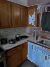
\includegraphics{kitchenShrunkframes0}\\
Frame 1\\
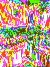
\includegraphics{kitchenShrunkframes1}\\
Frame 2\\
\end{center}

\section{Other rules, shapes, and sizes}

The codeword sets can be generated with an size array, with only size 4 being fully tested and 8 showing the same properties. Within this prototype project, calculation of truth table lengths of $2^{16}$ using all 4x4 binary grids are acceptable, lengths of $2^{64}$ using 8x8 grids would be challenging at this point. At size 8 there are $2^8=256$ possible codewords, which means that while you can't calculate the whole truth table at once you can calculate the codewords for any input individually on the spot. The codeword set's uniqueness and distribution properties seem to apply at size 8 by testing random codeword input tiles; it is only exhaustively tested for size 4. The internal hash logic transforms can also still be easily calculated for size 8 because you only have to work with codewords rather than the entire set of inputs. Future iterations of the project may implement input tile rectangles.\\

Out of the other 0-255 ECA rules, some do better than these particular 8 at lossy compression, losing only 3/16 bits instead of 6/16 bits with these 8. In particular the Pascal rules 90, 165, 102, 153, 105, 150 rank near the top, connected to several of these 10 via the property of XOR-additiveness \cite{xorAdditive}. However none outside of these 10 have unique solutions or even distributions in either row or column weighted, maxxed or minned.\\

\bibliographystyle{plain}
\bibliography{HashBib.bib}

\end{document}